\documentclass[../TDM3_courbe_app.tex]{subfiles}%

\begin{document}
\section[s]"1"{Projection de vecteurs}
\QR{%
	Exprimer $\vfo$ dans la base $(\ux,\uz)$ en fonction de $v_0$ et
	$\a$.
	\begin{center}
		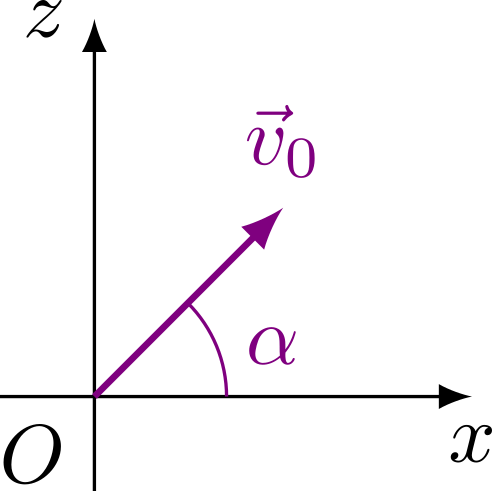
\includegraphics[scale=1]{vec_a}
	\end{center}
}{%
	Si $\a$ vaut 0, $\vfo$ est selon $\ux$. On sait donc que la
	projection de $\vfo$ sur $\ux$ donne $v_0\cos\a\ux$. On le remarque
	également avec le triangle rectangle OMH, avec M le bout de $\vfo$ et H
	son projeté orthogonal sur $\ux$~: la longueur OH est en effet
	$v_0\cos\a$. \bigbreak
	Si $\a$ vaut $\pi/2$, $\vfo$ est selon $\uz$. On sait donc que la
	projection de $\vfo$ sur $\uz$ donne $v_0\sin\a\uz$. On le remarque
	également en prenant le triangle rectangle OMJ, avec cette fois J le
	projeté orthogonal de M sur $\uz$~: la longueur OJ est en effet
	$v_0\sin\a$. Finalement,
	\[\boxed{\vfo = v_0\cos (\a)\,\ux + v_0\sin(\a)\,\uz}\]
}
\QR{%
	Exprimer $\Nf$ et $\Tf$ dans la base $(\ux,\,\uz)$ en fonction de $N$,
	$T$ et $\a$.
	\begin{center}
		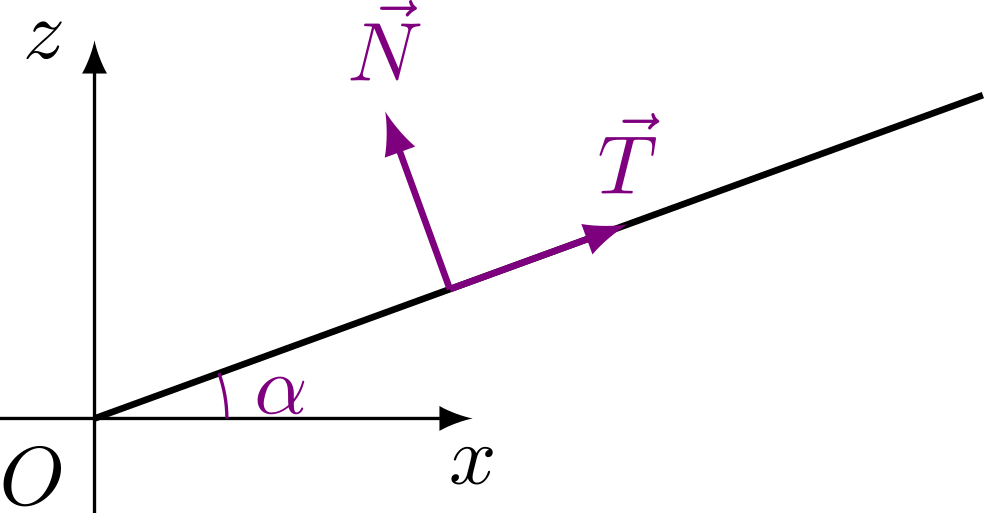
\includegraphics[scale=1]{vec_b}
	\end{center}
}{%
	Avec la même réflexion, on trouve
	\[\boxed{\Tf = T\cos(\a)\,\ux + T\sin(\a)\,\uz}\]
	La méthode est la même pour $\Nf$, mais le résultat est différent. En
	effet, si $\a = 0$, $\Nf$ est selon $\uz$~: la projection de $\Nf$ sur
	$\uz$ donne $N\cos\a\uz$. Si $\a = \pi/2$, $\Nf$ est selon $-\ux$~: la
	projection de $\Nf$ sur $\ux$ donne $-N\sin\a\ux$. Ainsi,
	\[\boxed{\Nf = -N\sin(\a)\,\ux + N\cos(\a)\,\uz}\]
}
\QR{%
	Exprimer $\Pf$ et $\Tf$ dans la base $(\er,\,\et)$ en fonction de $m$,
	$g$, $T$ et $\th$.
	\begin{center}
		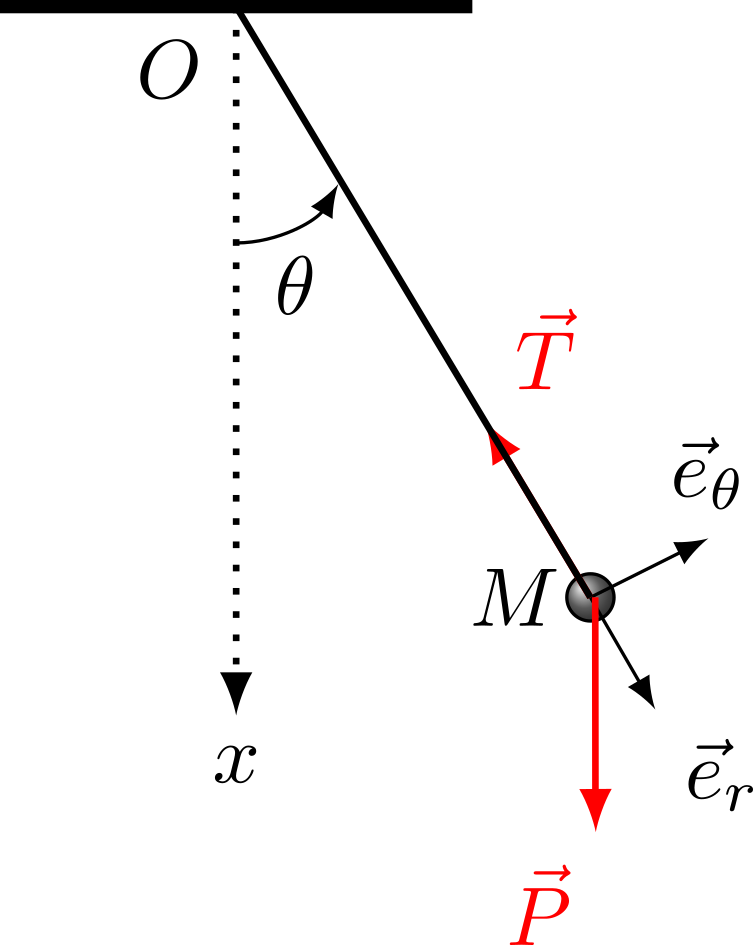
\includegraphics[scale=1]{vec_c}
	\end{center}
}{%
	Toujours même réflexion~: si $\th = 0$, $\Pf$ est selon $\er$, et si
	$\th = \pi/2$, $\Pf$ est selon $-\et$. $\Tf$ est, par définition, selon
	$-\er$. Ainsi,

	\[
		\boxed{\Pf = mg\cos(\th)\,\er -mg\sin(\th)\,\et}
		\qet
		\boxed{\Tf = -T\,\er}
	\]
}
\QR{%
	\textbf{Équilibre plan incliné}
	À l'équilibre des forces, on a
	\[\Nf + \Tf + \Pf = \of\]
	Projeter le poids dans la base inclinée et exprimer les normes de $\Tf$
	et $\Nf$ en fonction de $m$, $g$ et $\a$.
	\begin{center}
		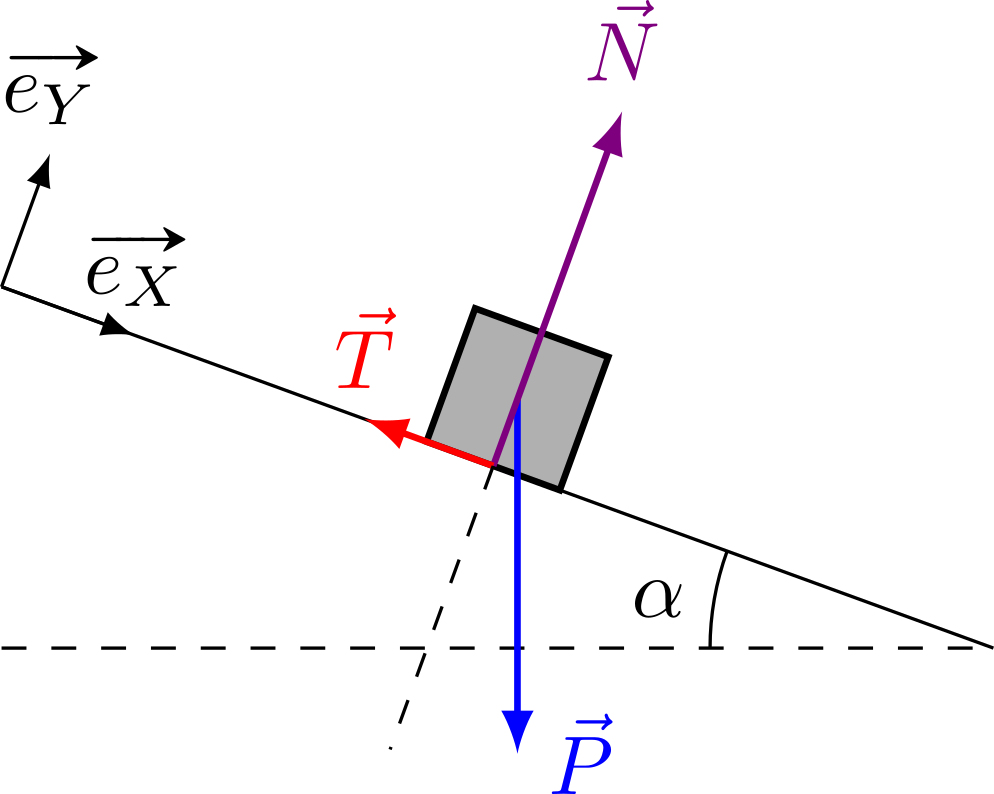
\includegraphics[scale=1]{vec_d}
	\end{center}
}{%
	Ici aussi~:
	\begin{itemize}
		\item $\a = 0 \Ra \Pf\cdot\vv{e_Y} = -1
			      \quad
			      \text{($\Pf$ selon $-\vv{e_Y}$)}$
		\item $\a = \pi/2 \Ra
			      \Pf\cdot\vv{e_X} = 1
			      \quad
			      \text{($\Pf$ selon $\vv{e_X}$)}$
	\end{itemize}
	Ainsi
	\[
		\boxed{\Pf = mg(\sin(\a)\,\vv{e_X} -\cos(\a)\,\vv{e_Y})}
		\qet
		\boxed{\Nf = N\,\vv{e_Y}}
		\qet
		\boxed{\Tf = -T\vv{e_X}}
	\]
	D'où
	\[
		\Nf + \Tf + \Pf = \of
		\Lra
		\mqty(mg\sin\a -T\\-mg\cos\a + N) = \mqty(0\\0)
		\Lra
		\boxed{
			\left\{
			\begin{aligned}
				T & = mg\sin\a \\
				N & = mg\cos\a
			\end{aligned}
			\right.}
	\]
}
\QR{%
	\textbf{Équilibre hamac}
	À l'équilibre des forces, on a
	\[\Ff_g + \Ff_d + \Pf = \of\]
	Projeter les vecteurs $\Ff_g$ et $\Ff_d$ dans la base $(\ux,\uy)$ avec
	$\ux$ parallèle au sol vers la droite et $\uy$ vertical ascendant. En
	déduire la norme littérale de ces deux vecteurs. On prend $m =
		\SI{60}{kg}$, $\a = \ang{45}$ et $\beta = \ang{60}$.
	\begin{center}
		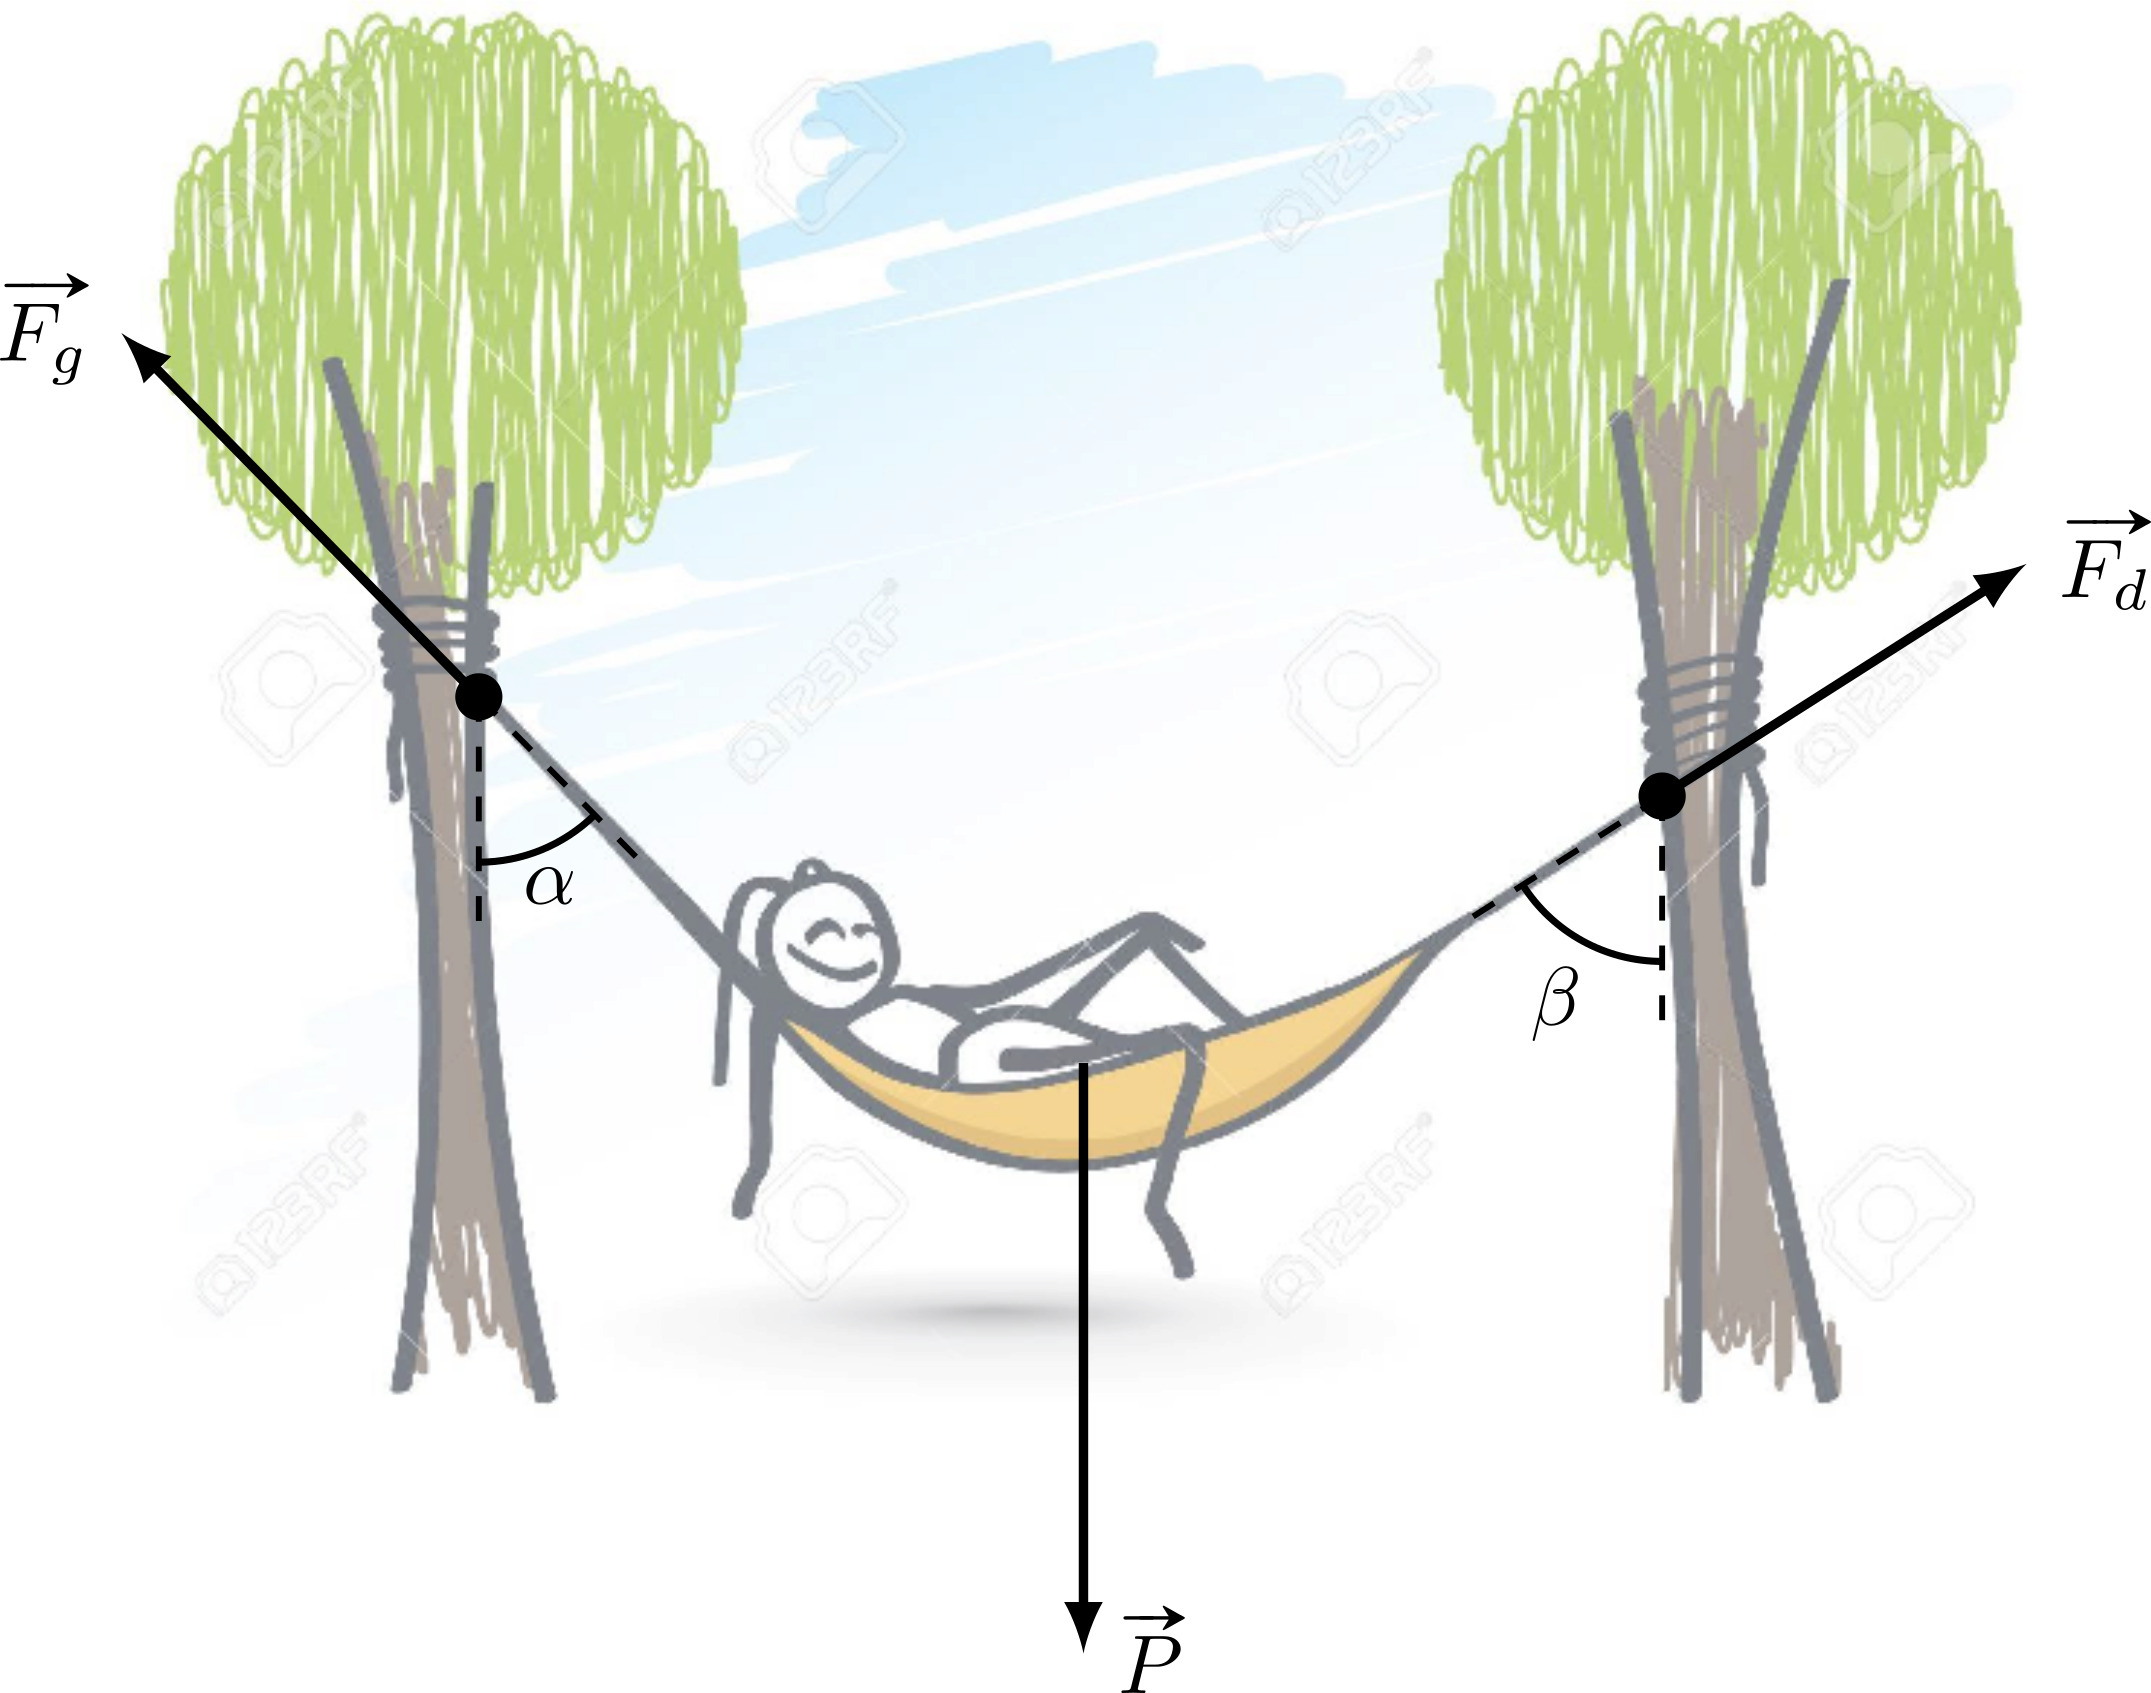
\includegraphics[scale=.7]{vec_e}
	\end{center}
}{%
	On projette~:
	\[
		\Ff_g = F_g(\cos\a\uy -\sin\a\ux)
		\qet
		\Ff_d = F_d(\cos\bb\uy+\sin\bb\ux)
	\]
	et avec l'égalité de vecteurs on obtient
	\begin{align*}
		\left\{
		\begin{aligned}
			0 & = F_d\sin\bb -F_g\sin\a      \\
			0 & = -mg+F_g\cos\a + F_d\cos\bb
		\end{aligned}
		\right.
		 & \Lra
		\left\{
		\begin{aligned}
			F_d & = F_g\frac{\sin\a}{\sin\bb}                    \\
			mg  & = F_g\cos\a + F_g\frac{\sin\a}{\sin\bb}\cos\bb
		\end{aligned}
		\right.
		\\\Lra
		\left\{
		\begin{aligned}
			F_d       & = F_g\frac{\sin\a}{\sin\bb}          \\
			mg\sin\bb & = F_g(\cos\a\sin\bb + \sin\a\cos\bb)
		\end{aligned}
		\right.
		 & \Lra
		\boxed{
			\left\{
			\begin{aligned}
				F_d & = \frac{mg\sin\a}{\cos\a\sin\bb + \sin\a\cos\bb}  \\
				F_g & = \frac{mg\sin\bb}{\cos\a\sin\bb + \sin\a\cos\bb}
			\end{aligned}
			\right.
		}
	\end{align*}
	Les applications numériques, \textbf{non demandées}, donnent
	\[
		\boxed{
			\left\{
			\begin{array}{rcl}
				F_d & = & \SI{4.4e2}{N} \\
				F_g & = & \SI{5.4e2}{N}
			\end{array}
			\right.
		}
	\]
}

\end{document}
